\section{CAnalytics Features}\label{canalytics-features}


% place system figure here simply for paper layout
\begin{figure*}
	\centering
	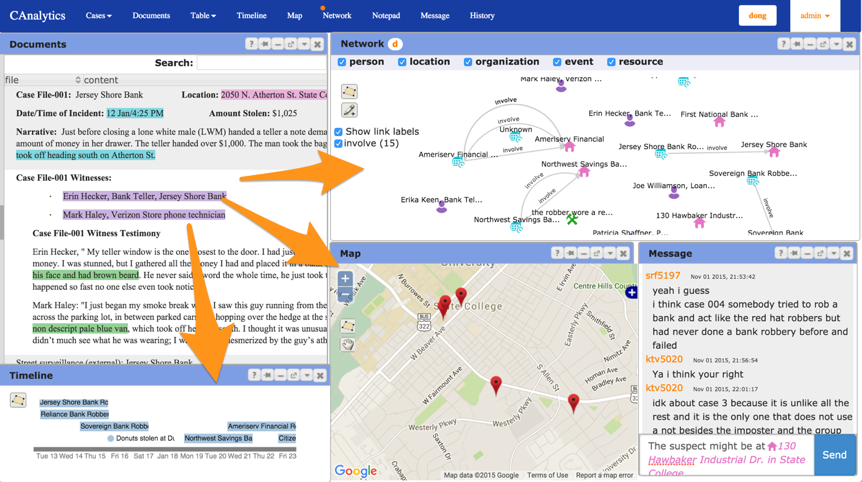
\includegraphics[width=\columnwidth]{./img/interface.png}
	\caption{CAnalytics user interface. Each window is closable, movable, and resizable. Shown here are \emph{document} view (top left), timeline (bottom left), network (top right), map (bottom middle), and message (bottom right). Other windows include table, notepad, and history view. }\label{fig:canalytics}
\end{figure*}

%\bvh{I think that the biggest thing missing from here is an argument about *why* they tool has been built the way it is. This should really link up to the arguments that you made in the abstract/intro about dynamism and collaboration more explicitly.}

As shown in Figure~\ref{fig:canalytics}, we developed a web application tool, \emph{CAnalytics} (standing for ``C-ollaborative Analytics''), to
support teams of analysts in identifying, visualizing, integrating and
assessing facts from multiple sources. Two particular design objectives are 1) to build an integrated environment for data modeling and analysis, and 2) to support collaboration with shared data and awareness functions. The design is informed by earlier
paper prototype studies \cite{Borge2012, Carroll2013}, in which the researchers examined team's communication patterns and
spontaneously created artifacts in a crime scenario. We also take into account findings from
empirical studies conducted by Chin et al. \cite{Chin2009} and Kang
and Stasko \cite{Kang2011} when making design decisions.
%\bvh{I would mention the reasons why we built it again here as an organizing structure for introducing the features and how they relate to those two overriding goals of dynamism and collaboration - modified}

\subsection{Coordinated multiple views for data modeling and analysis}

To enable an integrated environment for different functionalities of analysis, CAnalytics employs a multiple-view interface, with each view in a floating, closable window. Views are coordinated and share the underlying data pool so that products of different activities are not fragmented. The following paragraphs describe features of each view.

The \emph{document} view supports evidence modeling through annotation. Annotation provides a basic structure to assist analysts in containing and framing new data. In the
document view users can select and highlight a snippet of text and
annotate it as a type of entity such as a person, location, event, etc.,
or as a relationship between entities. Unlike other entity-based
systems such as \cite{Bier2010,Stasko2008}, we use annotations to
allow analysts to manually create evidence objects of interest. Manual
annotation allows for greater user control in terms of
information of interest and granularity that best suits their ad-hoc
analytic needs.
%\bvh{I wouldn't make too big of a point out of not supporting automated analysis, I would instead put it as something to look at in future work. You are sort of calling out a whole couple of fields in this set of statements. - modified}
Users can add attributes to the annotated object, e.g.~time in an event, and geo-coordination in a location. We can
also make reference to other objects in the attribute; for example,
adding people objects to an event indicating that these people
were involved in the event.
%\bvh{I almost think this is too fine grained of a description...you could just take the first sentence or two of this and add it to the previous paragraph. -deleted some}

These annotations turn text into structured data objects, which are then displayed in visualizations in the same workspace, including \emph{table}, \emph{timeline}, \emph{map},
and \emph{network} view---artifacts that are frequently constructed to hold attribute
data, temporal data, spatial data and relational data respectively
%\bvh{not sure what point you are trying to make here}
\cite{Carroll2013}. Figure~\ref{fig:canalytics} shows an example:
when an annotation is created in the document view with information
about time, location, participants, and their relationships, a new event
is created in the timeline view, a new location is created in the map
view, and new people are added to the network graph with a labeled edge
representing the relationship (or new edges are added to existing
nodes). Hovering the mouse over an entity will activate an entity detail
window that displays attributes in detail, and analysts can modify, or
re-model the entity in situ.

The views afford brushing and linking interactions;
that is, when users brush entities in one view, related
entities are displayed in other views. Thus the analyst can narrow down
entities to their interest by: specifying a time range using the functionality provided on the timeline; making a spatial query
with map filter; or selecting a cluster of entities by drawing a bounding
area in the network view.

\subsection{Collaboration and awareness features}

To support collaboration, CAnalytics affords real-time collaborative editing, similar to 
Google Tools. Users can open several concurrent editors to
collaboratively edit multiple entity objects. Entities and annotations are immediately
shared within a team and rendered in teammates' corresponding views.

In addition to real-time data sharing, CAnalytics supports other awareness features. A \emph{notification system} sends
individual's actions to the team in the form of a text box located in the top
right corner of the workspace. An iconic
indicator on top of a view window, which we call \emph{tool coordinator}, shows who else is also working on this view. A \emph{message} tool is a real time chat window that enables team
communication with persistent message history. The system also maintains
a traceable log of time-stamped individual activities in the \emph{history} tool.
Users can learn team activities about who did what to which object at
what time. Entities mentioned in the message tool and
history tool are hyperlinked and will trigger pop-up detail window when
the user moves the mouse over them. With these awareness features, users who work
synchronously can be informed of others' activity continuously; users
who work asynchronously will be able to use the history to reconstruct
their work status and become aware of changes beyond the point of their
last interaction.
